%-------------------------------------------------------------------
\chapter{Introduction}
\label{ch:intro}
%-------------------------------------------------------------------

This thesis is in the field of computer vision, specifically single image depth estimation.

\section{Background}
Under the name of "Depth Estimation" (DE) a lot of techniques appear, but there is no formal definition that considers them all.
DE could be defined as the study of algorithms that process one or more images of a scene and output information about its geometry.
There exist many approaches to do this as well as many problem settings.
The setting of this thesis is \textit{Single Image Depth Estimation} (SIDE), also called \textit{Monocular Depth Estimation} (MDE).
It refers to a depth estimation problem based on only one image of the scene.
As of today, this is done by assigning to each image pixel a depth value corresponding to the depth of the object that forms that pixel in the camera coordinate system.

\vspace{0.2cm}

\textbf{Images} are what we want to extract geometry information from.
Images will be indicated using the symbols $\mathbf{I}$ and $\mathbf{J}$.
From a computational point of view, images are tensors.
If $H$ and $W$ are respectively the height and width of a color image, then such an image is represented as an $H \times W \times 3$ shaped numerical tensor.
The last dimension of the tensor represents red, green and blue color intensities associated to each pixel.
Numerical values span in the range $[0, 1]$, hence an image $\mathbf{I}$ belongs to $[0, 1]^{H \times W \times 3}$.
A pixel is a location on an image and is indexed using a pair of integer numbers $(i, j)$.
Throughout this thesis, pixels will be indicated by the letter $p$.

\vspace{0.2cm}

\begin{figure}
    \centering
    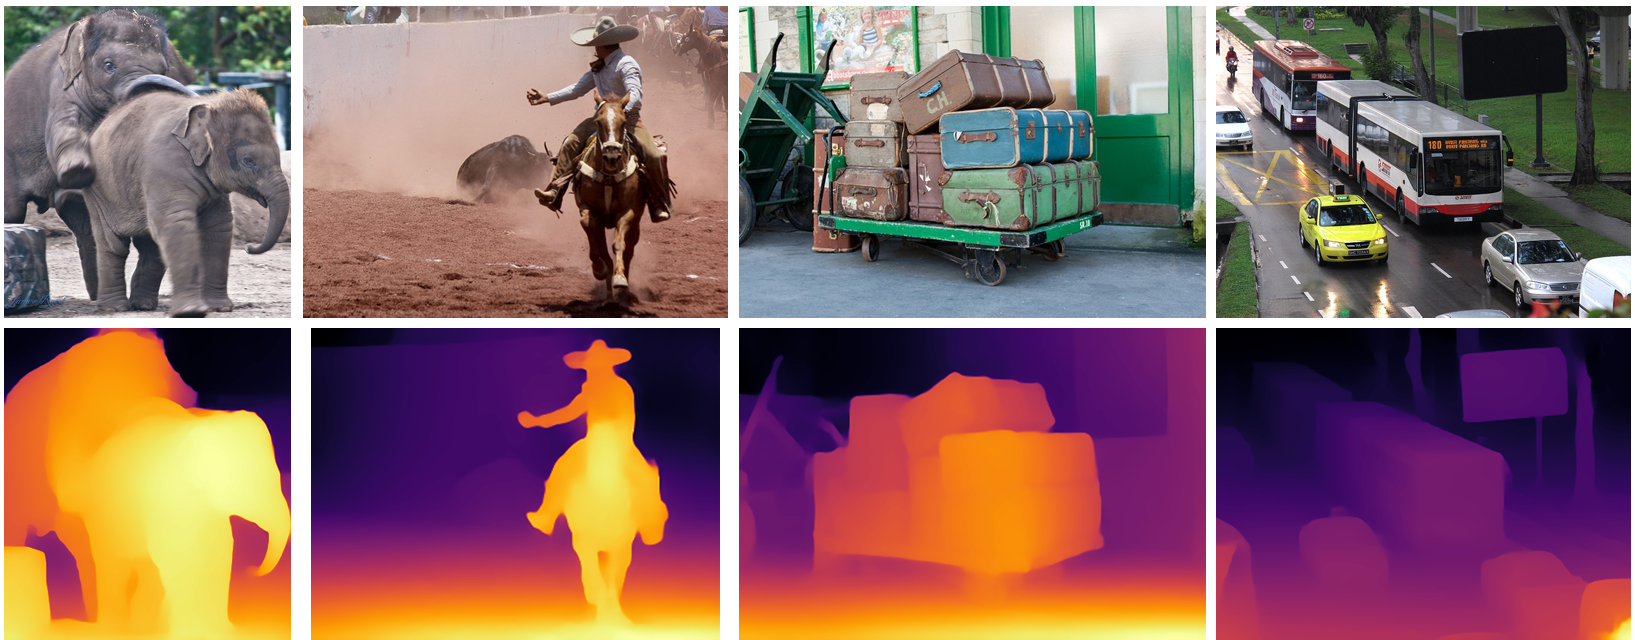
\includegraphics[scale=0.3]{figs/depth_maps_example}
    \caption{
        An example of images (top) and their depth maps (bottom).
        Depth values are color-coded: darker colors correspond to farther points in space.
        Figure taken from \cite{MiDas}.
        \label{fig:depth_maps_example}
    }
\end{figure}

\textbf{Depth maps} are the main output of depth estimation algorithms.
A depth map is an image in which every pixel value represents a depth measure, that is the $Z$ coordinate of the point $\mathbf{X} = (X, Y, Z)$ in space that corresponds to the pixel.
In figure \ref{fig:coordinates} the geometry of a simple image formation model is depicted and shows how the camera reference system is positioned.
Since only points in front of the camera are considered, $Z$ values are always strictly positive.
I will usually refer to a depth map using the symbol $\mathbf{Z}$.
\begin{figure}
    \centering
    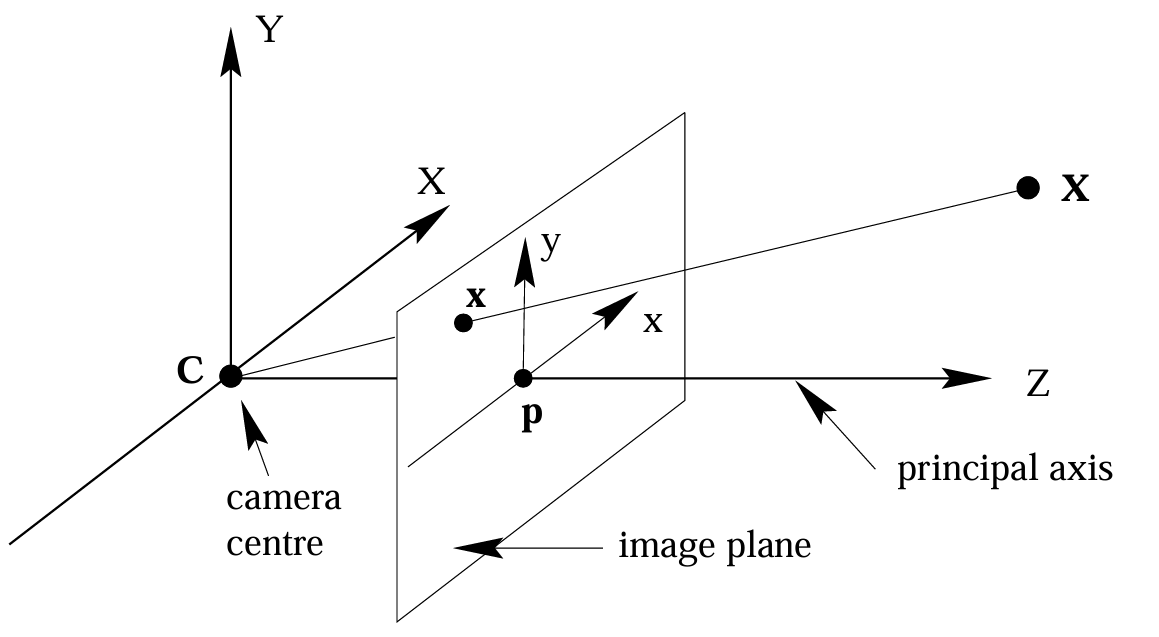
\includegraphics[scale=0.3]{figs/coordinates}
    \caption{
        Camera geometry, image from \cite{multiview}.
        The image plane reference system is defined by coordinates $x$ and $y$ which correspond to $j$ and $-i$.
        The point $\mathbf{p}$ is called the \textit{principal point} of the camera, it will appear in chapter \ref{ch:methods}.
        \label{fig:coordinates}
    }
\end{figure}

$\mathbf{Z}$ can be a \textit{metric} depth map, meaning each pixel value represents a spatial distance expressed in absolute physical units (e.g. meters), or it can be a \textit{relative} depth map and only used for relative depth comparisons of pairs of pixels (i.e. which pixel is closer or farther).
An important kind of relative depth map is the \textit{affine} depth map, that is a depth map equals to a metric one up to an affine transformation: $\mathbf{Z}_{\text{metric}} = s \, \mathbf{Z}_{\text{affine}} + t$ for some $s, t$.

Following an image formation model, in both images and depth maps every pixel value is determined by some property of a 3D scene location which I will denote as $\mathbf{X}$, be it distance, reflectance, color, texture or others.
The camera acquiring the image has \textit{intrinsic} parameters describing its acquisition geometry and \textit{extrinsic} ones referring to its position in space.
Projective geometry is used for expressing how points in space are mapped to the image plane \cite{multiview}.
If depth is known, also the opposite is possible.
This operation is called \textit{back-projection}.

\textbf{Disparity maps} are a concept related to the so-called \textit{stereo} or \textit{binocular} depth estimation where scene geometry must be inferred from two images.
Nevertheless, some MDE method predicts disparity maps instead of depth maps.
Disparity maps will be indicated by $\mathbf{D}$. In order to understand what they are, assume there is an object in the scene at $\mathbf{x}$ and two identical cameras simultaneously take a picture from slightly different angles.
The object location in the first image $(i_{1}, j_{1})$ will be different from its location in the second image $(i_{2}, j_{2})$ (imagine overlapping the two images).
A displacement $d = (i_{2} - i_{1}, j_{2} - j_{1})$ is thus obtained.
By knowing extrinsic and intrinsic parameters of the two cameras, depth $Z$ from the first camera (corresponding to $(i_{1}, j_{1})$) can be computed by means of such a displacement.

Thus, for every pixel $(i, j)$ of the first image, by back-projecting it in 3D space and then projecting it on the second image a displacement $\mathbf{D}(i,j)$ can be computed.
The mapping from pixel to displacement is called a disparity map, in this example we computed the disparity map of the first image w.r.t. the second.
Analogously a disparity map can be computed for the second image w.r.t. the first.
There exist pixels for which this procedure fails either because the projection of $\mathbf{x}$ onto the other image ends up out-of-view or because $\mathbf{x}$ is occluded from the other perspective and does not contribute to image formation.
Hence, disparity maps can have "holes" in which they are not defined.

In the very simple setting of identical cameras put side to side (mounted on a \textit{stereo-rig}) pointing at parallel directions, the disparity $d$ is a one dimensional displacement and is represented by a single real number.
This will be the case from here on. The obtained image pair is called \textit{rectified}.


The problem of depth estimation is to design an algorithm that can reconstruct the geometry of a scene from $N$ images of it.
A function $f$ is required such that $f(I_{1}, I_{2}, ..., I_{N})$ represents such geometry, usually as a depth map $\mathbf{Z}$ or disparity map $\mathbf{D}$, but other representations exist in particular when $N > 2$, i.e. \textit{multi-view} case.
There exist surveys treating the problem for $N \geq 2$ \cite{correspondance, stereo}, but the focus of this thesis is the case $N = 1$, namely \textit{monocular} or \textit{single image} depth estimation.


In the \textbf{deep learning} approach $f$ is called a $model$ and has \textit{trainable} parameters which must be tuned minimizing what is called a \textit{loss function} $\mathcal{L}$, that is: a quantity expressing some undesired property that $f$ mustn't satisfy.
For it to be minimized during a first phase called \textit{training}, differentiability of $\mathcal{L}$ in the trainable parameters is required.
This implies that $f$ itself should be differentiable in them.
Algorithms based on gradient descent are employed for optimization.
$\mathcal{L}$ is often expressed as a sum of other loss functions and so called \textit{regularization} terms which serve the overall training procedure, favouring the \textit{generalization} of the model.
A model is said to generalize well when its predictions are reliable on new input data, i.e. not seen during training.
This whole procedure is only possibile if a \textit{dataset} is given, that is a collection of data statistically defining the desired behaviour of $f$.
It can be a set of input-output pairs, e.g. images and associated depth maps, or a more general data collection, e.g. video footage.
The desired output of the model in response to a certain input is called \textit{ground-truth}.

\textit{Testing} follows training.
During the testing phase the model generalization capability is evaluated on new data using \textit{metrics} $\mathcal{M}$ which quantitatively express the \textit{error} the model is committing (like loss functions do, hence the smaller the better) or its \textit{accuracy} (the greater the better).
In order to test a model a dataset containing ground-truth data is necessary so that the desired behaviour can be quantitatively compared with the actual behaviour.
The output of a model is often called a \textit{prediction}, so metrics $\mathcal{M}$ are functions of both predictions and ground truth data.


\textit{Statistical learning} is the predecessor of deep learning and it shares with it the same theoretical foundations, but it proved to be less effective.
Deep learning efficacy is mainly due to its scalability in training, meaning that very large datasets can be used and the resulting optimization problem is computationally feasible for the existing hardware, although the costs are not always affordable.

%During testing time all monocular depth estimation models are able to infer depth from a single image, however during training the kind of data they require can vary from tecnique to tecnique.
%Chapter 2 treats these differences. In its "Supervised" section models trained on ground-truth data are presented, while in the "Self Supervised" one ground-truth is not necessary and data can be video footage or stereo pairs.
%Instead in "Classic" techniques not necessarily based on deep learning(and hence on datasets) are reviewed.
%
%In this chapter some of the ideas developed for solving monocular depth estimation are reviewed.
%The "Classic" section is about works that don't use what we'd call deep learning.
%"Supervised" , "Self Supervised" and in particular "SOTA" are solely about deep learning techniques.
%Datasets and metrics details are encapsulated in the "Datasets" and "Metrics" sections.
%
%
%I won't spend too much time on neural network architectures and in particular on explaining numerical details and experiments.
%If a method appears in this chapter it means that it was successful in its intent.
%The scale of efficacy is Classic $<$ Self Supervised $<$ Supervised $<$ SOTA.

Single Image Depth Estimation (SIDE) saw a growing research interest in the last years.
Its popularity is to be attributed to advancements in robotics and autonomous driving which could benefit from solving this task.
In fact, depth sensors are expensive and not reliable in various scenarios (for instance in presence of reflective surfaces).
Stereo rigs are instead difficult to use since constant calibration is required.
Hence, if depth could be accurately estimated by using only a single RGB camera, research in navigating real-world environments would be boosted.

Deep learning is the leading methodology for tackling SIDE.
The research trend is to train large models on various datasets to achieve zero-shot performances, meaning to generalize on unseen datasets.
MiDas~\cite{MiDas} was the leading work in this direction that managed to train a model on heterogeneous datasets.
It was done by converting each ground truth data to a common representation, in particular the authors chose to work in the disparity space.
The most common architecture is an encoder-decoder model that works at multiple scales.
The encoder is a classification backbone and the decoder estimates successive finer depth maps from the computed features of the encoder.
An example of such an architecture is illustrated in figure \ref{fig:flow_net}.
\begin{figure}
    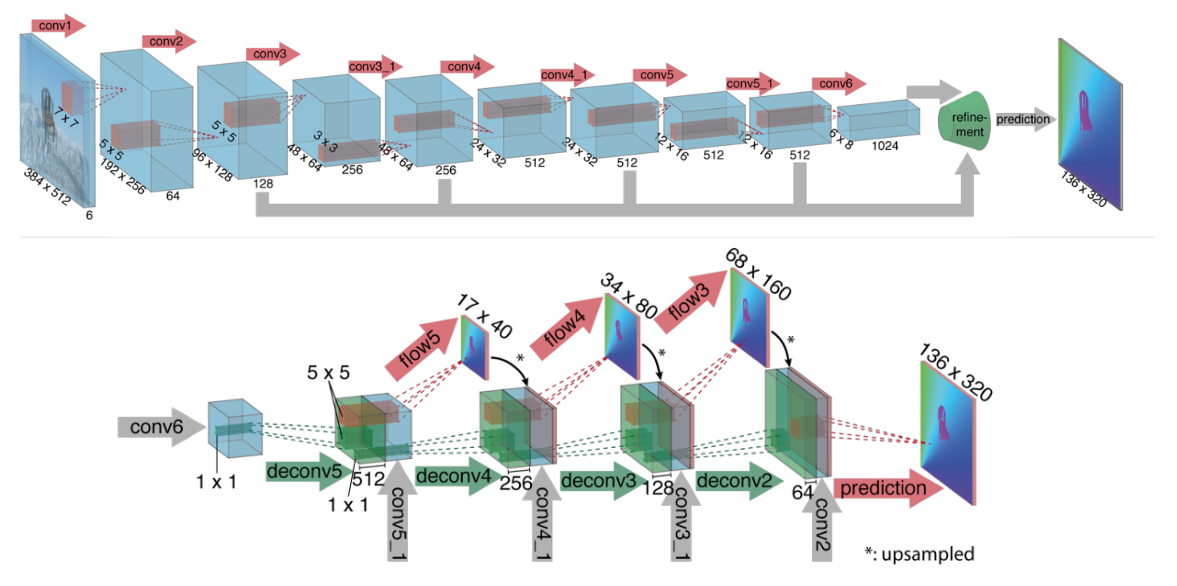
\includegraphics[scale=0.5]{figs/flow_net}
    \caption{
        FlowNet architecture from \cite{FlowNet}.
        At the top row the encoder is detailed, while the multi-scale decoder is shown at the bottom.
        This architecture was firstly used for optical flow estimation and later adapted to depth estimation (starting from \cite{DispNet}).
        \label{fig:flow_net}    
    }
\end{figure}
As noted by Bhat~et~al~\cite{ZoeDepth}, larger backbones achieve better metrics.
In recent years other architectures gained popularity, in particular transformer-based architectures \cite{denseViT, PatchFusion} and diffusion models.
Large Vision models (LVMs) are large neural networks trained on internet-scale data.
Ke et al. adapted and fine-tuned a LVM based on diffusion to perform SIDE.
The fine-tuning was performed on photo-realistic synthetic data and the resulting model showed zero-shot state of the art performances on various real world datasets.

These works are opposed to the needs of robotics and autonomous driving.
In such applications large neural networks present various problems.
For instance, performing real-time inference on edge devices could be prohibitive.
Most importantly, deep learning models are well known to be black-boxes.
Their functioning is not understood by humans (it is \textit{opaque}), this fact represents a problem in a sensitive application like driving.
With the growing diffusion of neural network based software in society, its interaction with consumers and the need for regulatory laws, being able to understand and interpret these algorithms is a necessity.
Explainable Artificial Intelligence (XAI) deals with this problem by developing methods for explaining deep learning models behavior~\cite{XAI_review}.
Despite the popularity of XAI in the research community, only few works address the problem of explainability in SIDE~\cite{Hu, Dijk, towards_interpretable}.

Objective of this thesis is to investigate the concept of interpretability, central to XAI, and its relation to SIDE.
It is shown that some XAI research methods are biased and that there exist theoretical limitations to explainability that have consequences on the whole field of research.
In particular, it is argued that solving SIDE implies a minimum degree of opaqueness and that non-interpretable methods must be used to some extent.

To reduce the impact of black-box methods on the overall interpretability of a SIDE pipeline, the idea of simplifying a learning problem is introduced.
Toy experiments test this approach applied to patch-wise depth estimation.
Results suggest that this practice can be beneficial.

The rest of the thesis is organized as follows:
\begin{itemize}
    \item{
        Chapter \ref{ch:sota} reviews various methods for SIDE.
        Treated methods span from early days to most recent developments.
        The last two sections are about XAI and works on interpretability of SIDE models.
    }
    \item{
        Chapter \ref{ch:methods} addresses the problem of interpretability from a theoretical point of view.
        The above claims about interpretability are supported in sections \ref{sec:limits of XAI}, \ref{sec:limits of interpretability} and \ref{sec:interpretability of depth estimation}.
        In section \ref{sec:hybrid}, the formal theory of learning is quickly reviewed and possible simplifications to the problem of patch-wise depth estimation are presented and motivated.
        The last section \ref{sec:depth_fusion} proposes a design for an interpretable algorithm that stitch together the partial estimates from the previous section.
    }
    \item{
        Chapter \ref{ch:results} presents and comments the experimental results obtained with the simplifications discussed in section \ref{sec:hybrid}.
    }
    \item{
        Chapter \ref{ch:conc} closes this thesis by summing up its contributions and suggestions for future work.
    }
\end{itemize}